\documentclass[10pt]{book}

\usepackage[utf8]{inputenc}
\usepackage[english]{babel}
\usepackage[T1]{fontenc}

\usepackage{calc}  % To compute length of line (used in Description)
\usepackage{enumitem}
\usepackage{comment}
\usepackage{authblk} % For affiliation / institute
\usepackage{booktabs} % lines in tables

%%% Math
\usepackage{amsfonts}
\usepackage{amsthm}
\usepackage{amsmath}
\usepackage{amssymb}

%%% Symbols
\newcommand{\uv}{\mathbf{u}}    % u vector
\newcommand{\ev}{\mathbf{e}}    % e vector
\newcommand{\vv}{\mathbf{v}}    % v vector
\newcommand{\NN}{\mathrm{NN}}

%%% Algorithms
\usepackage{algorithm}
\usepackage{algcompatible}
\usepackage{algpseudocode}
\renewcommand{\Comment}[2][.525\linewidth]{%
  \leavevmode\hfill\makebox[#1][l]{$\triangleright$~#2}} % To align the comments

%%% Graphics
\usepackage[hyperref]{xcolor} % (option that determine which other packages are to be loaded or supported)
\usepackage{graphicx} % For logos
\usepackage{marvosym} % Smile

%%% Index | To be loaded before hyperref
\usepackage{imakeidx}
\makeindex[intoc]

%%% Hyperref configuration
\PassOptionsToPackage{hyphens}{url}\usepackage{hyperref} % to break the links
\hypersetup{
    colorlinks=true,
    linkcolor=blue,  % color of internal links
    urlcolor=blue,   % color of external links
    citecolor=blue,  % color of links to bibliography
}

%%% Metadata
\title{\rule{\textwidth}{0.4pt}\\\huge{An algorithmic reasoning\\approach to GNNs}\\\rule{\textwidth}{0.4pt}}
\author{\Large{Angela Carraro}}
\author{\Large{Matteo Scorcia}}
\affil{\Large{DSSC + IN20 - UniTS}}
\date{}


%%% Chapter/sections/etc visual style 
% Redefine \marginpar with custom style
\let\defaultmarginpar\marginpar
\renewcommand\marginpar[2][]{\defaultmarginpar{\itshape\color{gray}#2}}
% Paragraph style
%\setlength{\parindent}{0pt}
\setlength{\parskip}{4pt}


\begin{document}

\begin{minipage}[c][\textheight]{\textwidth}
    \maketitle
    
    \hspace*{20cm}

    \centering
    
\includegraphics[height=2.5cm]{figures/logo_dssc_alt.pdf}
    \hspace*{1cm}
    
\includegraphics[height=2.5cm]{figures/Logo_units_blu.pdf}

\end{minipage}
\newpage

\tableofcontents

\newpage

\chapter{Graph Representation Learning}

Summary of \cite{BookHamiltonGRL}.

\section{Introduction}
\label{sec:intro}

Graphs are a widespread data structure and a universal language for describing complex systems. In the most general view, a graph is simply a collection of objects (i.e., nodes), along with a set of interactions (i.e., edges) between pairs of these objects.

The power of the graph formalism lies both in its focus on \emph{relationships between points} (rather than the properties of individual points), as well as in its generality.


\subsection{What is a graph?}

Before we discuss machine learning on graphs, it is necessary to give a bit more formal description of what exactly we mean by ``graph data''\index{graph data}. Formally, a \emph{graph}\index{graph}\marginpar{graph} $G = (V, E)$ is defined by a set of nodes $V$ and a set of edges $E$ between these nodes. We denote an edge going from node $u \in V$ to node $v \in V$ as $(u, v) \in E$. In many cases we will be concerned only with \emph{simple graphs}, where there is at most one edge between each pair of nodes, no edges between a node and itself, and where the edges are all undirected, i.e., $(u, v) \in E \Longleftrightarrow  (v, u) \in E$.

A convenient way to represent graphs is through an \emph{adjacency matrix}\index{adjacency matrix}\marginpar{adjacency matrix} $A \in
\mathbb R^{|V| \times |V|}$. To represent a graph with an adjacency matrix, we order the nodes in the graph so that every node indexes a particular row and column in the adjacency matrix. We can then represent the presence of edges as entries in this matrix: $A[u, v] = 1$ if $(u, v) \in E$ and $A[u, v] = 0$ otherwise. If the graph contains only undirected edges then $A$ will be a symmetric matrix, but if the graph is directed (i.e., edge direction matters) then A will not necessarily be symmetric. Some graphs can also have weighted edges, where the entries in the adjacency matrix are arbitrary real-values rather than $\{0, 1\}$.

Beyond the distinction between undirected, directed and weighted edges, we will also consider graphs that have different types of edges. In these cases we can extend the edge notation to include an edge or relation type $\tau$, e.g., $(u, \tau, v) \in E$, and we can define one adjacency matrix $A_\tau$ per edge type. We call such graphs \emph{multi-relational}\index{multi-relational graph}\marginpar{multi-relational graph}, and the entire graph can be summarized by an adjacency tensor $\mathcal A \in \mathbb R^{|V| \times |\mathcal R| \times |V|}$, where $\mathcal R$ is the set of relations.

Lastly, in many cases we also have \emph{attribute} or \emph{feature} information associated with a graph. Most often these are node-level attributes that we represent using a real-valued matrix $X \in \mathbb R^{|V| \times m}$, where we assume that the ordering of the nodes is consistent with the ordering in the adjacency matrix. In some cases we even associate real-valued features with entire graphs.

\subsection{Machine learning on graphs}

\subsubsection{Node classification}

In \emph{node classification}\index{node classification}\marginpar{node classification} the goal is to predict
the label $y_u$ --- which could be a type, category, or attribute --- associated with all the nodes $u \in V$, when we are only given the true labels on a training set of nodes $V_\text{train} \subset V$. Node classification is perhaps the most popular machine learning task on graph data, especially in recent years.

At first glance, node classification appears to be a straightforward variation of standard supervised classification, but there are in fact important differences. The most important difference is that the nodes in a graph are not \emph{independent and identically distributed (i.i.d.)}\marginpar{nodes not i.i.d.}. Usually, when we build supervised machine learning models we assume that each datapoint is statistically \emph{independent} from all the other datapoints; otherwise, we might need to model the dependencies
between all our input points. We also assume that the datapoints are \emph{identically distributed}; otherwise, we have no way of guaranteeing that our model will generalize to new datapoints. Node classification completely breaks this i.i.d. assumption. Rather than modeling a set of i.i.d. datapoints, we are instead modeling an interconnected set of nodes.

In fact, the key insight behind many of the most successful node classification approaches is to explicitly leverage the connections between nodes. One particularly popular idea is to exploit \emph{homophily}\index{homophily}\marginpar{homophily}, which is the tendency for nodes to share attributes with their neighbors in the graph. Based on the notion of homophily we can build machine learning models that try to assign similar labels to neighboring nodes in
a graph. Beyond homophily there are also concepts such as
\emph{structural equivalence}\index{structural equivalence}\marginpar{structural equivalence}, which is the idea that nodes with similar local neighborhood structures will have similar labels, as well as \emph{heterophily}\index{heterophily}\marginpar{heterophily}, which presumes that nodes will be preferentially connected to nodes with different labels. For example, gender is an attribute that exhibits heterophily in many social networks (boys want to connect to girls and vice versa). When we build node classification models we want to exploit these concepts and model the relationships between nodes, rather than simply treating nodes as independent datapoints.

\textbf{Supervised or semi-supervised?} Due to the atypical nature of node classification, researchers often refer to it as semi-supervised. This terminology is used because when we are training node classification models, we usually have access to the full graph, including all the unlabeled (e.g., test) nodes. The only thing we are missing is the labels of test nodes. However, we can still use information about the test nodes (e.g., knowledge of their neighborhood in the graph) to improve our model during training. This is different from the usual supervised setting, in which unlabeled datapoints are completely unobserved during training.

The general term used for models that combine labeled and unlabeled
data during training is semi-supervised learning, so it is understandable that this term is often used in reference to node classification tasks. It is important to note, however, that standard formulations of semi-supervised learning still require the i.i.d. assumption, which does not hold for node classification. Machine learning tasks on graphs do not easily fit our standard categories! 

\subsubsection{Edge prediction}

Node classification is useful for inferring information about a node based on its relationship with other nodes in the graph. But what about cases where we are missing this relationship information? Can we use machine learning to infer the edges between nodes in a graph?
This task goes by many names, such as link prediction, graph completion, and relational inference, depending on the specific application domain. We will simply call it \emph{edge prediction}\index{edge prediction}\marginpar{edge prediction} here. Along with node classification, it is one of the more popular machine learning tasks with graph data and has countless real-world applications: recommending content to users in social platforms, predicting drug side-effects, or inferring new
facts in a relational databases --- all of these tasks can be
viewed as special cases of relation prediction.

The standard setup for relation prediction is that we are given a set of nodes $V$ and an incomplete set of edges between these nodes $E_\text{train} \subset E$. Our goal is to use this partial information to infer the missing edges $E \ E_\text{train}$.  Like node classification, relation prediction blurs the boundaries of traditional machine learning categories --- often being referred to as both supervised and unsupervised --- and it requires inductive biases that are specific to the graph domain.

\subsubsection{Clustering and community detection}

Both node classification and relation prediction require inferring \emph{missing} information about graph data, and in many ways, those two tasks are the graph analogues of supervised learning. \emph{Community detection}\index{community detection}\marginpar{community detection}, on the other hand, is the graph analogue of unsupervised clustering. The challenge of community detection is to infer latent community structures given only the input graph $G = (V, E)$.

\subsubsection{Graph classification, regression, and clustering}

In these \emph{graph classification or regression}\index{graph classification or regression}\marginpar{graph classification or regression} applications, we seek to learn over graph data, but instead of making predictions over the individual components of a single graph (i.e., the nodes or the edges), we are instead given a dataset of \emph{multiple different graphs} and our goal is to make independent predictions specific to each graph. In the related task of \emph{graph clustering}\index{graph clustering}\marginpar{graph clustering}, the goal is to learn an unsupervised measure of similarity between pairs of graphs.

Of all the machine learning tasks on graphs, graph regression and classification are perhaps the most straightforward analogues of standard supervised learning. Each graph is an i.i.d. datapoint associated with a label, and the goal is to use a labeled set of training points to learn a mapping from datapoints (i.e., graphs) to labels. In a similar way graph clustering is the straightforward extension of unsupervised clustering for graph data. The challenge in
these graph-level tasks, however, is how to define useful features that take into account the relational structure within each datapoint.

\section{Background and Traditional
Approaches}

\subsection{Graph Statistics and Kernel Methods}

\subsubsection{Node-level statistics and features}

In principle the properties and statistics we discuss below could be used as features in a node classification model (e.g., as input to a logistic regression model). We consider some features that could be used to differentiate the nodes in a network, and the properties we discuss are generally useful across a wide variety of node classification tasks.
\smallskip

\textbf{Node degree}

The most obvious and straightforward node feature to examine is the \emph{degree}\index{degree}\marginpar{degree}, which is usually denoted $d_u$ for a node $u \in V$ and simply counts the number of edges incident to a node:
\begin{equation}
    d_u = \sum_{v \in V} A[u, v].
    \label{eq:degree}
\end{equation}
Note that in cases of directed graphs, one can differentiate between
different notions of degree --- e.g., corresponding to outgoing edges or incoming edges by summing over rows or columns in \autoref{eq:degree}. In general, the degree of a node is an essential statistic to consider, and it is often one of the most informative features in traditional machine learning models applied to node-level tasks.
\smallskip

\textbf{Node centrality}

Node degree simply measures how many neighbors a node has, but this is not necessarily sufficient to measure the \emph{importance} of a node in a graph. In many cases we can benefit from additional and more powerful measures of node importance. To obtain a more powerful measure of importance, we can consider various measures of what is
known as \emph{node centrality}\index{node centrality}\marginpar{node centrality}, which can form useful features in a wide variety of node classification tasks.

One popular and important measure of centrality is the so-called \emph{eigenvector centrality}\index{eigenvector centrality}\marginpar{eigenvector centrality}. Whereas degree simply measures how many neighbors each node has, eigenvector centrality also takes into account how important a node's neighbors are. In particular, we define a node's eigenvector centrality $e_u$ via a recurrence relation in which the node's centrality is proportional to the average centrality of its neighbors:
\begin{equation}
    e_u = \frac1\lambda \sum_{v \in V} A[u, v] e_v \qquad \forall u \in V,
    \label{eq:eigencentr}
\end{equation}
where $\lambda$ is a constant. Rewriting this equation in vector notation with $\mathbf e$ as the vector of node centralities, we can see that this recurrence defines the standard eigenvector equation for the adjacency matrix:
\begin{equation}
    \lambda \mathbf e = A \mathbf e.
\end{equation}
In other words, the centrality measure that satisfies the recurrence in \autoref{eq:eigencentr} corresponds to an eigenvector of the adjacency matrix. Assuming that we require positive centrality values, we can apply the Perron-Frobenius Theorem --- for our purposes the key assertion in the theorem is that any irreducible
square matrix has a unique largest real eigenvalue, which is the only eigenvalue whose corresponding eigenvector can be chosen to have strictly positive components---  to further determine that the vector of centrality values $\mathbf e$ is given by the eigenvector corresponding to the largest eigenvalue of $A$.

One view of eigenvector centrality is that it ranks the likelihood that a node is visited on a random walk of infinite length on the graph. This view can be illustrated by considering the use of power iteration to obtain the eigenvector centrality values. That is, since $\lambda$ is the leading eigenvector of $A$, we can compute $\mathbf e$ using power iteration via2
\begin{equation}
    \mathbf e^{(t+1)} = A \mathbf e^{(t)}.
\end{equation}
If we start off this power iteration with the vector $\mathbf e^{(0)} = (1, 1, \ldots, 1)^T$, then we can see that after the first iteration $\mathbf e^{(1)}$ will contain the degrees of all the nodes. In general, at iteration $t \ge 1$, $\mathbf e^{(t)}$ will contain the number of length-$t$ paths arriving at each node. Thus, by iterating this process indefinitely we obtain a score that is proportional to the number of times a node is visited on paths of
infinite length. This connection between node importance, random walks, and the spectrum of the graph adjacency matrix will return often throughout the ensuing sections and chapters of this book.
\smallskip

\textbf{The clustering coefficient}

The \emph{clustering coefficient}\index{clustering coefficient}\marginpar{clustering coefficient} measures the proportion of closed triangles in a node's local neighborhood. The popular \emph{local variant} of the clustering coefficient is computed as follows:
\begin{equation}
    c_u = \frac{|(v_1, v_2) \in E: v_1, v_2 \in \mathcal N(u)|}{\binom{d_u}2}.
\end{equation}
The numerator in this equation counts the number of edges between neighbours of node $u$ (where we use $\mathcal N(u) = \{v \in V: (u, v) \in E\}$ to denote the node neighborhood). The denominator calculates how many pairs of nodes there are in $u$'s neighborhood. The clustering coefficient takes its name from the fact that it measures how
tightly clustered a node's neighborhood is. A clustering coefficient of $1$ would imply that all of $u$'s neighbors are also neighbors of each other.

\subsubsection{Graph-level features and graph kernels}

So far we have discussed various statistics and properties at the node level, which could be used as features for node-level classification tasks. However, what if our goal is to do graph-level classification? Many of the methods we survey here fall under the general classification of \emph{graph kernel methods}\index{graph kernel methods}, which are approaches to designing features for graphs or implicit kernel functions that can be used in machine learning models.
\smallskip

\textbf{Bag of nodes}

The simplest approach to defining a graph-level feature is to just aggregate node-level statistics. For example, one can compute histograms or other summary statistics based on the degrees, centralities, and clustering coefficients of the nodes in the graph. This aggregated information can then be used as a graph-level representation. The downside to this approach is that it is entirely based upon local node-level information and can miss important global properties in the graph.
\smallskip

\textbf{The Weisfeiler-Lehman kernel}

One way to improve the basic bag of nodes approach is using a strategy of \emph{iterative neighborhood aggregation}\index{iterative neighborhood aggregation}. The idea with these approaches is to extract node-level features that contain more information than just their local ego graph, and then to aggregate these richer features into a graph-level representation.

Perhaps the most important and well-known of these strategies is the WeisfeilerLehman (WL) algorithm and kernel.

\subsection{Neighborhood Overlap Detection}
\label{sec:neighovdet}

In the last section we covered various approaches to extract features or statistics about individual nodes or entire graphs. These node and graph-level statistics are useful for many classification tasks. However, they are limited in that they do not quantify the \emph{relationships} between nodes. For instance, the statistics discussed in the last section are not very useful for the task of relation prediction, where our goal is to predict the existence of an edge between two nodes.

In this section we will consider various statistical measures of neighborhood overlap between pairs of nodes, which quantify the extent to which a pair of nodes are related. For example, the simplest \emph{neighborhood overlap measure}\index{neighborhood overlap measure}\marginpar{neighborhood overlap measure} just counts the number of neighbors that two nodes share:
\begin{equation}
    \mathbf S[u, v] = |\mathcal N(u) \cap \mathcal N(v)|,
\end{equation}
where we use $\mathbf S[u, v]$ to denote the value quantifying the relationship between nodes $u$ and $v$ and let $\mathbf S \in \mathbb R^{|V| \times |V|}$ denote the \emph{similarity matrix}\index{similarity matrix}\marginpar{similarity matrix} summarizing all the pairwise node statistics.

Even though there is no ``machine learning'' involved in any of the statistical measures discussed in this section, they are still very useful and powerful baselines for relation prediction. Given a neighborhood overlap statistic $\mathbf S[u, v]$, a common strategy is to assume that the likelihood of an edge $(u, v)$ is simply
proportional to $\mathbf S[u, v]$:
\begin{equation}
    \mathbf P (A[u, v] = 1) \propto \mathbf S[u, v].
\end{equation}
Thus, in order to approach the relation prediction task using a neighborhood overlap measure, one simply needs to set a threshold to determine when to predict the existence of an edge. Note that in the relation prediction setting we generally assume that we only know a subset of the true edges $E_\text{train} \subset E$. Our hope is that \emph{node-node similarity measures}\index{node-node similarity measures}\marginpar{node-node similarity measures} computed on the training edges will lead to accurate predictions about the existence of test (i.e., unseen) edges.

\subsection{Towards Learned Representations}

In the previous sections, we saw a number of traditional approaches to learning over graphs. However, the approaches discussed in
this chapter|and especially the node and graph-level statistics|are limited due to the fact that they require careful, hand-engineered statistics and measures.  The following chapters in this book introduce alternative approach to learning over graphs: \emph{graph representation learning}. Instead of extracting hand-engineered features, we will seek to \emph{learn} representations that encode structural information about the graph.


\section{Neighborhood Reconstruction Methods}

This part of the book is concerned with methods for learning node embeddings. The goal of these methods is to encode nodes as low-dimensional vectors that summarize their graph position and the structure of their local graph neighborhood. In other words, we want to project nodes into a latent space, where geometric relations in this latent space correspond to relationships (e.g., edges) in the original graph or network (\autoref{fig:nodeembedding}).

\begin{figure}[ht]
    \centering
    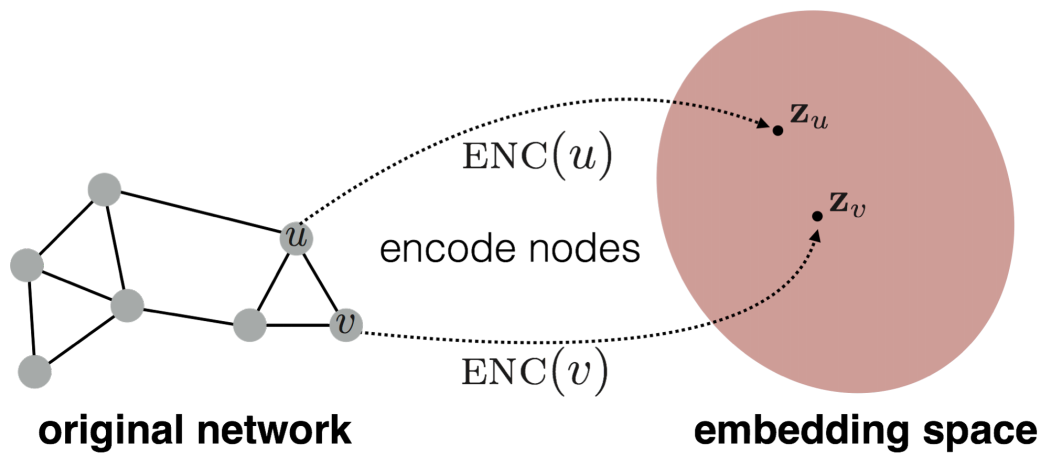
\includegraphics[width=8cm]{figures/Node_embedding.png}
    \caption{Illustration of the node embedding problem. Our goal is to learn an encoder (enc), which maps nodes to a low-dimensional embedding space. These embeddings are optimized so that distances in the embedding space reflect the relative positions of the nodes in the original graph.}
    \label{fig:nodeembedding}
\end{figure}

\subsection{An Encoder-Decoder Perspective}

We organize our discussion of node embeddings based upon the framework of \emph{encoding and decoding graphs}\index{encoding and decoding graphs}\marginpar{encoding and decoding graphs}. This way of viewing graph representation learning will reoccur throughout the book, and our presentation of node embedding methods based on this perspective closely follows \cite{Hamilton2018Representation}.

In the encoder-decoder framework, we view the graph representation learning problem as involving two key operations. First, an \emph{encoder}\index{encoder} model maps each node in the graph into a low-dimensional vector or embedding. Next, a \emph{decoder}\index{decoder} model takes the low-dimensional node embeddings and uses them to reconstruct information about each node's neighborhood in the original graph. This idea is summarized in \autoref{fig:enc-dec}.

\begin{figure}[ht]
    \centering
    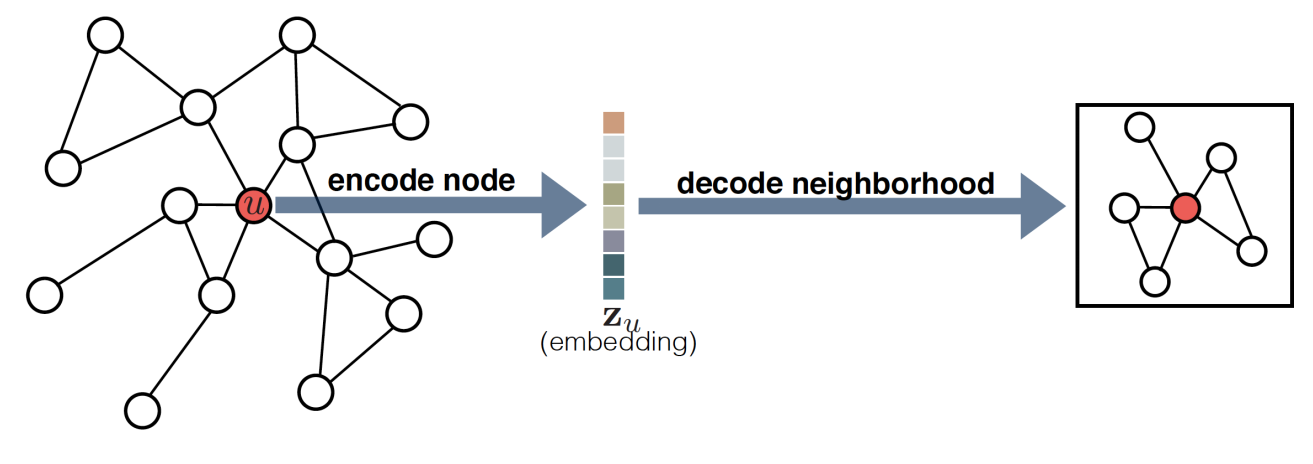
\includegraphics[width=10cm]{figures/Encoder_decoder.png}
    \caption{Overview of the encoder-decoder approach. The encoder maps the node $u$ to a low-dimensional embedding $\mathbf z_u$. The decoder then uses $\mathbf z_u$ to reconstruct $u$'s local neighborhood information.}
    \label{fig:enc-dec}
\end{figure}

\subsubsection{The Encoder}

Formally, the \emph{encoder}\index{encoder}\marginpar{encoder} is a function that maps nodes $v \in V$ to vector embeddings $\mathbf z_v \in \mathbb R^d$ (where $\mathbf z_v$ corresponds to the embedding for node $v \in V$). In the simplest case, the encoder has the following signature:
\begin{equation}
    \textsc{enc}: V \rightarrow \mathbb R^d,
\end{equation}
meaning that the encoder takes node IDs as input to generate the node embeddings. In most work on node embeddings, the encoder relies on what we call the \emph{shallow embedding}\index{shallow embedding}\marginpar{shallow embedding} approach, where this encoder function is simply an embedding lookup based on the node ID. In other words, we have that
\begin{equation}
    \textsc{enc}(v) = \mathbf Z[v],
    \label{eq:shallowemb}
\end{equation}
where $\mathbf Z \in \mathbb R^{|V| \times d}$ is a matrix containing the embedding vectors for all nodes and $\mathbf Z[v]$ denotes the row of $\mathbf Z$ corresponding to node $v$.

\subsubsection{The Decoder}

The role of the \emph{decoder}\index{decoder}\marginpar{decoder} is to reconstruct certain graph statistics from the node embeddings that are generated by the encoder. For example, given a node embedding $\mathbf z_u$ of a node $u$, the decoder might attempt to predict $u$'s set of neighbors $\mathcal N(u)$ or its row $A[u]$ in the graph adjacency matrix.

While many decoders are possible, the standard practice is to define pairwise decoders, which have the following signature:
\begin{equation}
    \textsc{dec}: \mathbb R^d \times \mathbb R^d \rightarrow \mathbb R^+.
\end{equation}
Pairwise decoders can be interpreted as predicting the relationship or similarity between pairs of nodes. For instance, a simple pairwise decoder could predict whether two nodes are neighbors in the graph.

Applying the pairwise decoder to a pair of embeddings $(\mathbf z_u, \mathbf z_v)$ results in the \emph{reconstruction} of the relationship between nodes $u$ and $v$. The goal is optimize the encoder and decoder to minimize the reconstruction loss so that
\begin{equation}
    \textsc{dec}(\textsc{enc}(u), \textsc{enc}(v)) = \textsc{dec}(\mathbf z_u, \mathbf z_v) \approx \mathbf S[u, v].
    \label{eq:reconstrloss}
\end{equation}
Here, we assume that $\mathbf S[u, v]$ is a graph-based similarity measure between nodes. For example, the simple reconstruction objective of predicting whether two nodes are neighbors would correspond to $\mathbf S[u, v] := A[u, v]$. However, one can define $\mathbf S[u, v]$ in more general ways as well, for example, by leveraging any of the pairwise neighborhood overlap statistics discussed in \autoref{sec:neighovdet}.


\subsubsection{Optimizing an Encoder-Decoder Model}

To achieve the reconstruction objective (\autoref{eq:reconstrloss}), the standard practice is to minimize an empirical reconstruction loss $\mathcal L$ over a set of training node pairs $\mathcal D$:
\begin{equation}
    \mathcal L = \sum_{(u,v) \in \mathcal D} \ell (\textsc{dec}(\mathbf z_u, \mathbf z_v), \mathbf S[u, v]),
    \label{eq:loss}
\end{equation}
where $\ell: \mathbb R \times \mathbb R \rightarrow \mathbb R$ is a loss function measuring the discrepancy between the decoded (i.e., estimated) similarity values $\textsc{dec}(\mathbf z_u, \mathbf z_v)$ and the true values $\mathbf S[u, v]$. Depending on the definition of the decoder ($\textsc{dec}$) and similarity function ($\mathbf S$), the loss function $\ell$ might be a mean-squared error or even a classification loss, such as cross entropy. Thus, the overall objective is to train the encoder and the decoder so that pairwise node relationships can be effectively reconstructed on the training set $\mathcal D$. Most approaches minimize the loss in \autoref{eq:loss} using stochastic gradient descent, but there are certain instances when more specialized optimization methods (e.g., based on matrix factorization) can be used.

\subsubsection{Overview of the Encoder-Decoder Approach}

\autoref{tab:shallowembalg} applies this encoder-decoder perspective to summarize several well-known node embedding methods|all of which use the shallow encoding approach. The key benefit of the encoder-decoder framework is that it allows one to succinctly define and compare different embedding methods based on (i) their decoder function, (ii) their graph-based similarity measure, and (iii) their loss function.

\begin{table}[ht]
    \centering
    \begin{tabular}{cccc}
        \toprule
        Method &  Decoder $\textsc{dec}(\mathbf{z}_u, \mathbf{z}_v)$ & Similarity measure $\mathbf S[u,v]$ & Loss function $\mathcal L$ \\
        \midrule
        Lap. Eigenmaps & $\|\mathbf{z}_u - \mathbf{z}_v\|_2^2$ & general & $\textsc{dec}(\mathbf{z}_u, \mathbf{z}_v)\cdot \mathbf S[u,v]$ \\
        
        Graph Fact. & $\mathbf{z}_u^T \mathbf{z}_v$ & $A[u,v]$ & $\|\textsc{dec}(\mathbf{z}_u, \mathbf{z}_v) \cdot \mathbf S[u,v]\|^2_2$ \\
        
        GraRep & $\mathbf{z}_u^T \mathbf{z}_v$ & $A[u,v],\ldots,A^k[u,v]$ & $\|\textsc{dec}(\mathbf{z}_u, \mathbf{z}_v) \cdot \mathbf S[u,v]\|^2_2$ \\
        
        HOPE & $\mathbf{z}_u^T \mathbf{z}_v$ & general & $\|\textsc{dec}(\mathbf{z}_u, \mathbf{z}_v) \cdot \mathbf S[u,v]\|^2_2$ \\
        
        DeepWalk & $\frac{e^{\mathbf{z}_u^T \mathbf{z}_v}}{\sum_{k \in V} e^{ \mathbf{z}_u^T \mathbf{z}_k}}$ & $p_G(v|u)$ & $- \mathbf S[u,v] \log(\textsc{dec}(\mathbf{z}_u, \mathbf{z}_v))$ \\
        
        node2vec & $\frac{e^{\mathbf{z}_u^T \mathbf{z}_v}}{\sum_{k \in V} e^{ \mathbf{z}_u^T \mathbf{z}_k}}$ & $p_G(v|u)$ (biased) & $- \mathbf S[u,v] \log(\textsc{dec}(\mathbf{z}_u, \mathbf{z}_v))$ \\
        \bottomrule
    \end{tabular}
    \caption{A summary of some well-known shallow embedding algorithms. Note that the decoders and similarity functions for the random-walk based methods are asymmetric, with the similarity function $p_G(v|u)$ corresponding to the probability of visiting $v$ on a fixed-length random walk starting from $u$.}
    \label{tab:shallowembalg}
\end{table}

\subsection{Limitations of Shallow Embeddings}

This focus of this chapter has been on shallow embedding methods. In these approaches, the encoder model that maps nodes to embeddings is simply an embedding lookup (\autoref{eq:shallowemb}), which trains a unique embedding for each node in the graph. However, it is also important to note that shallow embedding approaches suffer from some important drawbacks:
\begin{enumerate}
    \item The first issue is that they do not share any parameters between nodes in the encoder, since the encoder directly optimizes a unique embedding vector for each node. This lack of parameter sharing is both statistically and computationally inefficient.
    \item A second key issue is that they do not leverage node features in the encoder.
    \item Lastly --- and perhaps most importantly --- they are inherently \emph{transductive}\index{transductive}. These methods can only generate embeddings for nodes that were present during the training phase. Generating embeddings for new nodes|which are observed after the training phase|is not possible unless additional optimizations are performed to learn the embeddings for these nodes. This restriction prevents shallow embedding methods from being used on \emph{inductive}\index{inductive} applications, which involve generalizing to unseen nodes after training.
\end{enumerate}

To alleviate these limitations, shallow encoders can be replaced with more sophisticated encoders that depend more generally on the structure and attributes of the graph. We will discuss the most popular paradigm to define such encoders, i.e.., graph neural networks (GNNs).


\section{The Graph Neural Network Model}
\label{sec:GNNmodel}

The first part of this book discussed approaches for learning low-dimensional embeddings of the nodes in a graph. The node embedding approaches we discussed used a shallow embedding approach to generate representations of nodes, where we simply optimized a unique embedding vector for each node. In this chapter, we turn our focus to more complex encoder models. We will introduce the graph neural network (GNN) formalism, which is a general framework for defining deep neural networks on graph data. The key idea is that we want to generate representations of nodes that actually depend on the structure of the graph, as well as any feature information we might have.

The primary challenge in developing complex encoders for graph-structured data is that our usual deep learning toolbox does not apply. For example, convolutional neural networks (CNNs) are well-defined only over grid-structured inputs (e.g., images), while recurrent neural networks (RNNs) are well-defined only over sequences (e.g., text). To define a deep neural network over general graphs, we need to define a new kind of deep learning architecture.

\textbf{Permutation invariance and equivariance} One reasonable idea for
defining a deep neural network over graphs would be to simply use the
adjacency matrix as input to a deep neural network. For example, to generate an embedding of an entire graph we could simply flatten the adjacency
matrix and feed the result to a multi-layer perceptron (MLP):
\begin{equation}
    \mathbf z_G = \text{MLP}(\mathbf A[1] \oplus \mathbf A[2] \oplus \ldots \oplus \mathbf A[|\mathcal V|]);
\end{equation}
where $\mathbf A[i] \in \mathbf R^{|\mathcal V|}$ denotes a row of the adjacency matrix and we use $\oplus$ to denote vector concatenation.

The issue with this approach is that it \textit{depends on the arbitrary ordering of nodes that we used in the adjacency matrix}. In other words, such a model is not \textit{permutation invariant}, and a key desideratum for designing neural networks over graphs is that they should permutation invariant (or equivariant). In mathematical terms, any function f that takes an adjacency matrix $\mathbf A$ as input should ideally satisfy one of the two following properties:
\begin{align}
    f(\mathbf{PAP}^T) = f(\mathbf A) \qquad &\text{(Permutation Invariance)} \\
    f(\mathbf{PAP}^T) = \mathbf P f(\mathbf A) \qquad &\text{(Permutation Equivariance)},
\end{align}
where $\mathbf P$ is a permutation matrix. Permutation invariance means that the function does not depend on the arbitrary ordering of the rows/columns in the adjacency matrix, while permutation equivariance means that the output of $f$ is permuted in an consistent way when we permute the adjacency matrix. (The shallow encoders are an example of permutation equivariant functions.) Ensuring invariance or equivariance is a key challenge when we are learning over graphs, and we will revisit issues surrounding permutation equivariance and invariance often in the ensuing chapters.

\subsection{Neural Message Passing}

The defining feature of a GNN is that it uses a form of neural message passing in which vector messages are exchanged between nodes and updated using neural networks.

In the rest of this chapter, we will detail the foundations of this neural message passing framework. We will focus on the message passing framework itself and defer discussions of training and optimizing GNN models to the next Section. The bulk of this section will describe how we can take an input graph $G = (V, E)$,
along with a set of node features $\mathbf X \in \mathbb R^{d \times |V|}$, and use this information to generate node embeddings $\mathbf z_u, \forall u \in V$. However, we will also discuss how the GNN framework can be used to generate embeddings for subgraphs and entire
graphs.

During each message-passing iteration in a GNN, a \emph{hidden embedding}\index{hidden embedding}\marginpar{hidden embedding} $\mathbf h^{(k)}_u$ corresponding to each node $u \in \mathcal V$ is updated according to information aggregated from $u$'s graph neighborhood $\mathcal N(u)$. This message-passing update can be expressed as follows:
\begin{align}
    \mathbf h^{(k+1)}_u &= \textsc{update}^{(k)} \left( \mathbf h^{(k)}_u; \textsc{aggregate}^{(k)}(\{\mathbf h^{(k)}_v, \forall v \in \mathcal N(u)\}) \right) 
    \label{eq:mess-pass} \\
    &= \textsc{update}^{(k)} \left( \mathbf h^{(k)}_u, \mathbf m^{(k)}_{\mathcal N(u)} \right),
    \label{eq:mess-pass2}
\end{align}
where $\textsc{update}$ and $\textsc{aggregate}$ are arbitrary differentiable functions (i.e., neural networks) and $\mathbf m_{\mathcal N(u)} = \textsc{aggregate}(\{\mathbf h_v, \forall v \in \mathcal N(u)\})$ is the ``message'' that is aggregated from $u$'s graph neighborhood $\mathcal N(u)$. We use superscripts to distinguish the embeddings and functions at different iterations of message passing. The different iterations of message passing are also sometimes known as the different ``layers'' of the GNN.

At each iteration $k$ of the GNN, the $\textsc{aggregate}$ function takes as input the set of embeddings of the nodes in $u$'s graph neighborhood $\mathcal N(u)$ and generates a message $\mathbf m^{(k)}_{\mathcal N(u)} = \textsc{aggregate}^{(k)}(\{\mathbf h^{(k)}_v, \forall v \in \mathcal N(u)\})$ based on this aggregated neighborhood information. The update function $\textsc{update}$ then combines the message $\mathbf m^{(k)}_{\mathcal N(u)}$ with the previous embedding $\mathbf h^{(k−1)}_u$ of node $u$ to generate the updated embedding $\mathbf h^{(k)}_u$. The initial embeddings at k = 0 are set to the input features for all the nodes, i.e., $\mathbf h^{(0)}_u = \mathbf x_u, \forall u \in \mathcal V$. After running $K$ iterations of the GNN message passing, we can use the output of the final layer to define the embeddings for each node, i.e.,
\begin{equation}
    \mathbf z_u = \mathbf h^{(K)}_u, \forall u \in \mathcal V.
\end{equation}
Note that since the $\textsc{aggregate}$ function takes a set as input, GNNs defined in this way are permutation equivariant by design.

In cases where no node features are available, there are still several options. One option is to use node statistics to define
features. Another popular approach is to use identity features, where we associate each node with a one-hot indicator feature, which uniquely identifies that node. Note, however, that the using identity features makes the model transductive\index{transductive} and incapable of generalizing to unseen nodes.

The basic intuition behind the GNN message-passing framework is straightforward: at each iteration, every node aggregates information from its local neighborhood, and as these iterations progress each node embedding contains more and more information from further reaches of the graph.

But what kind of ``information'' do these node embeddings actually encode? Generally, this information comes in two forms. On the one hand there is \emph{structural information}\index{structural information}\marginpar{structural information} about the graph. For example, after $k$ iterations of GNN message passing, the embedding $\mathbf h^{(k)}_u$ of node $u$ might encode information about
the degrees of all the nodes in $u$'s $k$-hop neighborhood.

In addition to structural information, the other key kind of information captured by GNN node embedding is \emph{feature-based}\index{feature-based}\marginpar{feature-based}. After $k$ iterations of GNN message passing, the embeddings for each node also encode information about all the features in their $k$-hop neighborhood. This local feature-aggregation behaviour of GNNs is analogous to the behavior of the convolutional kernels in convolutional neural networks (CNNs). However, whereas CNNs aggregate
feature information from spatially-defined patches in an image, GNNs aggregate information based on local graph neighborhoods.

\subsubsection{The Basic GNN}

So far, we have discussed the GNN framework in a relatively abstract fashion as a series of message-passing iterations using \textsc{update} and \textsc{aggregate} functions (\autoref{eq:mess-pass}). In order to translate the abstract GNN framework defined in \autoref{eq:mess-pass} into something we can implement, we must give concrete instantiations to these \textsc{update} and \textsc{aggregate} functions. We begin here with the most basic GNN framework. The basic GNN message passing is defined as
\begin{equation}
    \mathbf h^{(k)}_u = \sigma \left( \mathbf W^{(k)}_\text{self} \mathbf h_u^{(k-1)} + \mathbf W_\text{neigh}^{(k)} \sum_{v \in \mathcal N(u)} \mathbf h^{(k-1)}_v + \mathbf b^{(k)} \right),
\end{equation}
where $\mathbf W^{(k)}_\text{self}, \mathbf W_\text{neigh}^{(k)} \in \mathbb R^{d^{(k)} \times d^{(k-1)}}$ are trainable parameter matrices and $\sigma$ denotes an elementwise non-linearity (e.g., a tanh or ReLU). The bias term $b^{(k)} \in \mathbb R^{d^{(k)}}$ is often omitted for notational simplicity, but including the bias term can be important to achieve strong performance. In this equation --- and throughout the remainder of the review --- we use superscripts to differentiate parameters, embeddings, and dimensionalities in different layers of the GNN.

The message passing in the basic GNN framework is analogous to a standard multi-layer perceptron (MLP) or Elman-style recurrent neural network, i.e., Elman RNN, as it relies on linear operations followed by a single elementwise non-linearity. We first sum the messages incoming from the neighbors; then, we combine the neighborhood information with the node's previous embedding using a linear combination; and finally, we apply an elementwise non-linearity.

We can equivalently define the basic GNN through the \textsc{update} and \textsc{aggregate} functions:
\begin{align}
    &\mathbf m_{\mathcal N(u)} = \sum_{v \in \mathcal N(u)} \mathbf h_v, 
    \label{eq:basicgnn} \\
    &\textsc{update}(\mathbf h_u, \mathbf m_{\mathcal N(u)}) = \sigma \left( \mathbf W_\text{self} \mathbf h_u + \mathbf W_\text{neigh} \mathbf m_{\mathcal N(u)} \right),
\end{align}
where we recall that we use
\begin{equation}
    \mathbf m_{\mathcal N(u)} = \textsc{aggregate}^{(k)}(\{ \mathbf h_v^{(k)}, \; \forall v \in \mathcal N(u)\})
\end{equation}
as a shorthand to denote the message that has been aggregated from $u$'s graph neighborhood. Note also that we omitted the superscript denoting the iteration in the above equations, which we will often do for notational brevity. In general, the parameters $\mathbf W_\text{self}, \mathbf W_\text{neigh}$ and $\mathbf b$ can be shared across the GNN message passing iterations or trained separately for each layer.

\textbf{Node vs. graph-level equations.} In the description of the basic GNN model above, we defined the core message-passing operations at the node level. However, it is important to note that many GNNs can also be succinctly defined using graph-level equations. In the case of a basic GNN, we can write the graph-level definition of the model as follows:
\begin{equation}
    \mathbf H^{(k)} = \sigma \left( A \mathbf H^{(k-1)} \mathbf W_\text{neigh}^{(k)} + \mathbf H^{(k-1)} \mathbf W_\text{self}^{(k)} \right),
\end{equation}
where $\mathbf H^{(k)} \in \mathbb R^{|V| \times d}$ denotes the matrix of node representations at layer $k$ in the GNN (with each node corresponding to a row in the matrix), $A$ is the graph adjacency matrix, and we have omitted the bias term for notational simplicity. While this graph-level representation is not easily applicable to all GNN models --- such as the attention-based models --- it is often more succinct and also highlights how many GNNs can be efficiently implemented using a small number of sparse matrix operations.

\subsubsection{Message Passing with Self-loops}

As a simplification of the neural message passing approach, it is common to add self-loops to the input graph and omit the explicit update step. In this approach we define the message passing simply as
\begin{equation}
    \mathbf h^{(k)}_u = \textsc{aggregate}(\{\mathbf h_v^{(k-1)}, \; \forall v \in \mathcal N(u) \cup \{u\}\}),
\end{equation}
where now the aggregation is taken over the set $\mathcal N(u) \cup \{u\}$, i.e., the node’s neighbors as well as the node itself. The benefit of this approach is that we no longer need to define an explicit update function, as the update is implicitly defined through the aggregation method.

In the case of the basic GNN, adding self-loops is equivalent to  sharing parameters between the $\mathbf W_\text{self}$ and $\mathbf W_\text{neigh}$ matrices, which gives the following graph-level update:
\begin{equation}
    \mathbf H^{(k)} = \sigma \left( (A + I) \mathbf H^{(k-1)} \mathbf W^{(k)} \right) .
\end{equation}
In the following chapters we will refer to this as the \emph{self-loop approach}\index{self-loop approach}\marginpar{self-loop approach}.

%\subsection{Generalized Neighborhood Aggregation}
\subsection{Graph convolutional networks (GCNs)}

%GCNN fatte con Generalized Neighborhood Aggregation. Poi si può fare anche Generalized Update Methods, che aiuta per l'oversmoothing.

The basic GNN can be improved upon and generalized in many ways: both the \textsc{aggregate} operator and the \textsc{update} can be generalized and improved upon.

The most basic neighborhood aggregation operation (\autoref{eq:basicgnn}) simply takes the sum of the neighbor embeddings. One issue with this approach is that it can be unstable and highly sensitive to node degrees. One solution to this problem is to simply \emph{normalize the aggregation operation} based upon the degrees of the nodes involved. The simplest approach is to just take an average rather than sum:
\begin{equation}
    \mathbf m_{\mathcal N(u)} = \frac{\sum_{v \in \mathcal N(u)} \mathbf h_v}{|\mathcal N(u)|},
\end{equation}
but researchers have also found success with other normalization factors, such as the following \emph{symmetric normalization}\index{symmetric normalization}\marginpar{symmetric normalization}:
\begin{equation}
    \mathbf m_{\mathcal N(u)} = \sum_{v \in \mathcal N(u)} \frac{\mathbf h_v}{\sqrt{|\mathcal N(u)| |\mathcal N(v)|}}.
\end{equation}

One of the most popular baseline graph neural network models --- the \emph{graph convolutional network (GCN)}\index{graph convolutional network (GCN)}\marginpar{graph convolutional network (GCN)} --- employs the symmetric-normalized aggregation as well as the self-loop approach\index{self-loop approach}. The GCN model thus defines the  message passing function as
\begin{equation}
    h^{(k)}_u = \sigma \left( \mathbf W^{(k)} \sum_{v \in \mathcal N(u) \cup \{u\}} \frac{\mathbf h_v}{\sqrt{|\mathcal N(u)| |\mathcal N(v)|}} \right).
\end{equation}

\textbf{To normalize or not to normalize?} Proper normalization can be essential to achieve stable and strong performance when using a GNN. It is important to note, however, that normalization can also lead to a loss of information. For example, after normalization, it can be hard (or even impossible) to use the learned embeddings to distinguish between nodes of different degrees, and various other structural graph features can be obscured by normalization. The use of normalization is thus an application-specific question. Usually, normalization is most helpful in tasks where node feature information is far more useful than structural information, or where there is a very wide range of node degrees that can lead to instabilities during optimization.

Neighborhood normalization can be a useful tool to improve GNN performance, but can we do more to improve the AGGREGATE operator? Is there perhaps something more sophisticated than just summing over the neighbor embeddings?

The neighborhood aggregation operation is fundamentally a set function. We are given a set of neighbor embeddings $\{\mathbf h_v, \forall v \in \mathcal N(u)\}$ and must map this set to a single vector $\mathbf m_{\mathcal N(u)}$. The fact that $\{\mathbf h_v, \forall v \in \mathcal N(u)\}$ is a set is in fact quite important: there is no natural ordering of a nodes’ neighbors, and any aggregation function we define must thus be permutation invariant.

One principled approach to define an aggregation function is based on the theory of permutation invariant neural networks. An aggregation function with the following form is a \emph{universal set function approximator}\index{universal set function approximator}\marginpar{universal set function approximator}:
\begin{equation}
    \mathbf m_{\mathcal N(u)} = \textbf{MLP}_\theta \left( \sum_{v \in \mathcal N(u)} \textbf{MLP}_\phi (\mathbf h_v) \right),
    \label{eq:univsetapproxf}
\end{equation}
where as usual we use $\textbf{MLP}_\theta$ to denote an arbitrarily deep multi-layer perceptron parameterized by some trainable parameters $\theta$. In other words, theoretical results show that any permutation-invariant function that maps a set of embeddings to a single embedding can be approximated to an arbitrary accuracy by a model following \autoref{eq:univsetapproxf}. Set pooling approaches based on \autoref{eq:univsetapproxf} often lead to small increases in performance, though they also introduce an increased risk of overfitting, depending on the depth of the MLPs used.

In addition to more general forms of set aggregation, a popular strategy for improving the aggregation layer in GNNs is to apply attention. The basic idea is to assign an attention weight or importance to each neighbor, which is used to weigh this neighbor’s influence during the aggregation step. The first GNN model to apply this style of attention was the Graph Attention Network (GAT), which uses attention weights to define a weighted sum of the neighbors:
\begin{equation}
    \mathbf m_{\mathcal N(u)} = \sum_{v \in \mathcal N(u)} \alpha_{u,v} \mathbf h_v,
\end{equation}
where $\alpha_{u,v}$ denotes the attention on neighbor $v \in \mathcal N(u)$ when we are aggregating information at node $u$. In the original GAT paper, the attention weights are defined as
\begin{equation}
    \alpha_{u,v} = \frac{\exp \left(\mathbf a^\top[\mathbf{Wh}_u \oplus \mathbf{Wh}_v] \right)}{\sum_{v' \in \mathcal N(u)} \exp \left( \mathbf a^\top [\mathbf{Wh}_u \oplus \mathbf{Wh}_{v'}] \right)},
\end{equation}
where $\mathbf a$ is a trainable attention vector, $\mathbf W$ is a trainable matrix, and $\oplus$ denotes the concatenation operation. Adding attention is a useful strategy for increasing the representational capacity of a GNN model, especially in cases where you have prior knowledge to indicate that some neighbors might be more informative than others. 

In many ways the \textsc{update} operator plays an equally important role as the \textsc{aggregate} operator in defining the power and inductive bias of the GNN model. So far, we have seen the basic GNN approach --- where the update operation involves a linear combination of the node’s current embedding with the message from its neighbors --- as well as the self-loop approach, which simply involves adding a self-loop to the graph before performing neighborhood aggregation. In
this section, we turn our attention to more diverse generalizations of the \textsc{update} operator.

\colorbox{yellow}{\ldots}

\subsection{Graph Pooling}

The neural message passing approach produces a set of node embeddings, but what if we want to make predictions at the graph level? In other words, we have been assuming that the goal is to learn node representations $\mathbf z_u, \; \forall u \in V$, but what if we to learn an embedding $\mathbf z_G$ for the entire graph $G$? This task is often referred to as \emph{graph pooling}\index{graph pooling}\marginpar{graph pooling}, since our goal is to pool together the node embeddings in order to learn an embedding of the entire graph.

Similar to the \textsc{aggregate} operator, the task of graph pooling can be viewed as a problem of learning over sets. We want to design a pooling function $f_p$, which maps a set of node embeddings $\{\mathbf z_1, \ldots, \mathbf z_{|V|} \}$ to an embedding $\mathbf z_G$ that represents the full graph.

There are two approaches that are most commonly applied for learning graph-level embeddings via set pooling. The first approach is simply
to take a sum (or mean) of the node embeddings:
\begin{equation}
    \mathbf z_G = \frac{\sum_{v \in V} \mathbf z_u}{f_n(|V|)},
\end{equation}
where $f_n$ is some normalizing function (e.g., the identity function, so $\mathbf z_G = (\sum_{v \in V} \mathbf z_u)/|V|$). While quite simple, pooling based on the sum or mean of the node embeddings is often sufficient for applications involving small graphs. The second popular set-based approach uses a combination of LSTMs and attention to pool the node embeddings (which we won't see).

One limitation of the set pooling approaches is that they do not exploit the structure of the graph. While it is reasonable to consider the task of graph pooling as simply a set learning problem, there can also be benefits from exploiting the graph topology at the pooling stage. One popular strategy to accomplish this is to perform \emph{graph clustering or coarsening}\index{graph clustering or coarsening} as a means to pool the node representations.

\subsection{Generalized Message Passing}

The presentation in this chapter so far has focused on the most popular style of GNN message passing, which operates largely at the node level. However, the GNN message passing approach can also be generalized to leverage edge and graph-level information at each stage of message passing. For example, in the more general approach proposed by \cite{battaglia2018relational}, we define each iteration of message passing according to the following equations:
\begin{align}
    \mathbf h^{(k)}_{(u,v)} &= \textsc{update}_\text{edge} (\mathbf h_{(u,v)}^{(k-1)}, \mathbf h_u^{(k-1)}, \mathbf h_v^{(k-1)}, \mathbf h_G^{(k-1)})
    \label{eq:upedge} \\
    \mathbf m_{\mathcal N(u)} &= \textsc{aggregate}_\text{node}(\{ \mathbf h_{(u,v)}^{(k)}, \; \forall v \in \mathcal N(u) \})
    \label{eq:message} \\
    \mathbf h^{(k)}_u &= \textsc{update}_\text{node} ( \mathbf h_u^{(k-1)}, \mathbf m_{\mathcal N(u)}, \mathbf h_G^{(k-1)})
    \label{eq:upnode} \\
    \mathbf h^{(k)}_G &= \textsc{update}_\text{graph}(\mathbf h_G^{( k-1)}, \{ \mathbf h_u^{(k)}, \, \forall u \in V\}, \{ \mathbf h_{(u,v)}^{(k)}, \forall (u, v) \in E\}).
    \label{eq:upgraph}
\end{align}
The important innovation in this generalized message passing framework is that, during message passing, we generate hidden embeddings $\mathbf h_{(u,v)}^{(k)}$ for each edge in the graph, as well as an embedding $h_G^{(k)}$ corresponding to the entire graph. This allows the message passing model to easily integrate edge and graph-level features, and recent work has also shown this generalized message passing approach to have benefits compared to a standard GNN in terms of logical expressiveness. Generating embeddings for edges and the entire graph during message passing also makes it trivial to define loss functions based on graph or edge-level classification tasks.

In terms of the message-passing operations in this generalized message-passing framework, we first update the edge embeddings based on the embeddings of their incident nodes (\autoref{eq:upedge}). Next, we update the node embeddings by aggregating the edge embeddings for all their incident edges (\autoref{eq:message} and \ref{eq:upnode}). The graph embedding is used in the update equation for both node and edge representations, and the graph-level embedding itself is updated by aggregating over all the node and edge embeddings at the end of each iteration (\autoref{eq:upgraph}). All of the individual update and aggregation operations in such a generalized message-passing framework can be implemented using the
techniques discussed earlier (e.g., using a pooling method to compute the graph-level update).


\section{Graph Neural Networks in Practice}

In \autoref{sec:intro}, we introduced a number of graph neural network (GNN) architectures. However, we did not discuss how these architectures are optimized and what kinds of loss functions and regularization are generally used. In this section, we will turn our attention to some of these practical aspects of GNNs. We will discuss some representative applications and how GNNs are generally optimized in practice, including a discussion of unsupervised pre-training methods that can be particularly effective. We will also introduce common techniques used to regularize and improve the efficiency of GNNs.

In the vast majority of current applications, GNNs are used for one of three tasks: node classification, graph classification, or relation prediction. As discussed in \autoref{sec:GNNmodel}, these tasks reflect a large number of real-world applications, such as predicting whether a user is a bot in a social network (node classification), property prediction based on molecular graph structures (graph classification), and content recommendation in online platforms (relation prediction). In this section, we briefly describe how these tasks translate into concrete loss functions for GNNs, and we also discuss how GNNs can be pre-trained in an unsupervised manner to improve performance on these downstream tasks.






\chapter{Graph Representation Learning - Video}

Notes of the video \cite{HamiltonGRLVideo}. Related video: \cite{PetarTF-GNN}.

Graphs are a general and universal language for describing and modelling complex systems/data.

In a graph setting, we are not considering a set of independent points, but really the whole object that we're trying to actually do learning upon is bound up in the interconnections or the relationships between these points. So rather than a set of individual data points we're considering the relationships between them.

Even trying to tell whether or not two graphs are the same is NP-indeterminate (it's believed not to be solved in polynomial time), since there is no standard or canonical way to order the nodes in the adjacency matrices (in a graph there is no up and down like in an image!).




\chapter{Relational inductive biases, deep learning, and graph networks}

Summary of \cite{battaglia2018relational}.

\section{Introduction}

A key signature of human intelligence is the ability to make ``infinite use of finite means'', in which a small set of elements (such as words) can be productively composed in limitless ways (such as into new sentences). This reflects the principle of \emph{combinatorial generalization}\index{combinatorial generalization}\marginpar{combinatorial generalization}, that is, constructing new inferences, predictions, and behaviors from known building blocks. Here we explore how to improve modern AI's capacity for combinatorial generalization by biasing learning towards structured representations and computations, and in particular, systems that operate on graphs. The question of how to build artificial systems which exhibit combinatorial generalization has been at the heart of AI since its origins, and was central to many structured approaches.

Recently, a class of models has arisen at the intersection of deep learning and structured approaches, which focuses on approaches for reasoning about explicitly structured data, in particular graphs. What these approaches all have in common is a capacity for performing computation over discrete entities and the relations between them. What sets them apart from classical approaches is how the representations and structure of the entities and relations --- and the corresponding computations --- can be learned, relieving the burden of needing to specify them in advance. Crucially, these methods carry strong \emph{relational inductive biases}\index{relational inductive bias}, in the form of specific architectural assumptions, which guide these approaches towards learning about entities and relations, which we, joining many others, suggest are an essential ingredient for human-like intelligence.

\section{Relational inductive biases}

We define \emph{structure}\index{structure} as the product of composing a set of known building blocks. ``Structured representations'' capture this composition (i.e., the arrangement of the elements) and ``structured computations'' operate over the elements and their composition as a whole. \emph{Relational reasoning}\index{relational reasoning}\marginpar{relational reasoning},
then, involves manipulating structured representations of \emph{entities} and \emph{relations}, using \emph{rules} for how they can be composed. We use these terms to capture notions from cognitive science, theoretical computer science, and AI, as follows:
\begin{itemize}
    \item An \emph{entity}\index{entity}\marginpar{entity} is an element with attributes, such as a physical object with a size and mass.
    \item A \emph{relation}\index{relation}\marginpar{relation} is a property between entities. Relations between two objects might include same size as, heavier than, and distance from. Relations can have attributes as well. The relation more than X times heavier than takes an attribute, X, which determines the relative weight threshold for the relation to be true vs. false. Relations can also be sensitive to the global context. For a stone and a feather, the relation falls with greater acceleration than depends on whether the context is in air vs. in a vacuum. Here we focus on pairwise relations between entities.
    \item A \emph{rule}\index{rule}\marginpar{rule} is a function (like a non-binary logical predicate) that maps entities and relations to other entities and relations, such as a scale comparison like is entity X large? and is entity X heavier than entity Y?. Here we consider rules which take one or two arguments (unary and binary), and return a unary property value.
\end{itemize}

An \emph{inductive bias}\index{inductive bias}\marginpar{inductive bias} allows a learning algorithm to prioritize one solution (or interpretation) over another, independent of the observed data. In a Bayesian model, inductive biases are typically expressed through the choice and parameterization of the prior distribution. In other contexts, an inductive bias might be a regularization term added to avoid overfitting, or it might be encoded in the architecture of the algorithm itself. Inductive biases often trade flexibility for improved sample complexity and can be understood in terms of the bias-variance tradeoff. Ideally, inductive biases both improve the search for solutions without substantially diminishing performance, as well as help find solutions which generalize in a desirable way; however, mismatched inductive biases can also lead to suboptimal performance by introducing constraints that are too strong.

Many approaches in machine learning and AI which have a capacity for relational reasoning use a \emph{relational inductive bias}\index{relational inductive bias}\marginpar{relational inductive bias}. While not a precise, formal definition, we use this term to refer generally to inductive biases  which impose constraints on relationships and interactions among entities in a learning process.

To explore the relational inductive biases expressed within various deep learning methods, we must identify several key ingredients: what are the \emph{entities}, what are the \emph{relations}, and what are the \emph{rules} for composing entities and relations, and computing their implications? In deep learning, the entities and relations are typically expressed as distributed representations, and the rules as neural network function approximators; however, the precise forms of the entities, relations, and rules vary between architectures. To understand these differences between architectures, we can further ask how each supports relational reasoning by probing:
\begin{itemize}
    \item The arguments to the rule functions (e.g., which entities and relations are provided as input).
    \item How the rule function is reused, or shared, across the computational graph (e.g., across different entities and relations, across different time or processing steps, etc.).
    \item How the architecture defines interactions versus isolation among representations (e.g., by applying rules to draw conclusions about related entities, versus processing them separately).
\end{itemize}

\subsection{Relational inductive biases in standard deep learning building blocks}

...

\section{Graph networks}

Models in the \emph{graph neural network}\index{graph neural network}\marginpar{graph neural networks} family have been explored in a diverse range of problem domains, across supervised, semi-supervised, unsupervised, and reinforcement learning settings. They have been effective at tasks thought to have rich relational structure, such as
\begin{itemize}
    \item visual scene understanding tasks and few-shot learning
    \item learn the dynamics of physical systems and multi-agent systems 
    \item reason about knowledge graphs
    \item predict the chemical properties of molecules
    \item predict traffic on roads
    \item classify and segment images and videos and 3D meshes and point clouds
    \item classify regions in images
    \item perform semi-supervised text classification
    \item machine translation
    \item combinatorial optimization
    \item boolean satisfiability
\end{itemize}

The works cited above are by no means an exhaustive list, but provide a representative cross-section of the breadth of domains for which graph neural networks have proven useful.

We now present our \emph{graph networks (GN)}\index{graph networks (GN)}\marginpar{graph networks (GN)} framework, which defines a class of functions for relational reasoning over graph-structured representations.  Note, we avoided using the term ``neural'' in the ``graph network'' label to reflect that they can be implemented with functions other than neural networks, though here our focus is on neural network implementations.

The main unit of computation in the GN framework is the GN block, a ``graph-to-graph'' module which takes a graph as input, performs computations over the structure, and returns a graph as output. As described in Box 3, entities are represented by the graph's nodes, relations by the edges, and system-level properties by global attributes.

\subsubsection{Definition of ``graph''}

Here we use ``graph'' to mean a directed, attributed multi-graph with a global attribute. In our terminology, a \emph{node}\index{node}\marginpar{node, edge, global attribute} is denoted as $\vv_i$, an \emph{edge}\index{edge} as $\ev_k$, and the \emph{global attributes}\index{global attribute} as $\uv$. We also use $s_k$ and $r_k$ to indicate the indices of the sender and receiver nodes (see below), respectively, for edge $k$.
To be more precise, we define these terms as:
\begin{description}[noitemsep, leftmargin=!,labelwidth=\widthof{\bfseries Global attribute}]
    \item[Directed:] one-way edges, from a ``sender'' node to a ``receiver'' node.
    \item[Attribute:] properties that can be encoded as a vector, set, or even another graph.
    \item[Attributed:] edges and vertices have attributes associated with them.
    \item[Global attribute:] a graph-level attribute.
    \item[Multi-graph:] there can be more than one edge between vertices, including self-edges.
\end{description}

Within our GN framework, a \emph{graph}\index{graph}\marginpar{graph} is defined as a 3-tuple $G = (\uv; V; E)$. The $\uv$ is a \emph{global attribute}\index{global attribute}; the $V = \{\vv_i \}_{i=1:N^v}$ is the \emph{set of nodes}\index{set of nodes} (of cardinality $N^v$), where each $\mathbf v_i$ is a node's attribute. The $E = \{(\ev_k; r_k; s_k)\}_{k=1:N^e}$ is the \emph{set of edges}\index{set of edges} (of cardinality $N^e$), where each $\ev_k$ is the edge's attribute, $r_k$ is the index of the receiver node, and $s_k$ is the index of the sender node.

\subsubsection{Internal structure of a GN block}

A GN block contains three ``update'' functions, $\phi$, and three ``aggregation'' functions, $\rho$,
\begin{align}
  \begin{split}
    \ev'_k &= \phi^e\left(\ev_k, \vv_{r_k}, \vv_{s_k}, \uv \right) \\
    \vv'_i &= \phi^v\left(\mathbf{\bar{e}}'_i, \vv_i, \uv \right) \\
    \uv' &= \phi^u\left(\mathbf{\bar{e}}', \mathbf{\bar{v}}', \uv \right)
  \end{split}
  \begin{split}
    \mathbf{\bar{e}}'_i &= \rho^{e \rightarrow v}\left(E'_i\right) \\
    \mathbf{\bar{e}}' &= \rho^{e \rightarrow u}\left(E'\right) \\
    \mathbf{\bar{v}}' &= \rho^{v \rightarrow u}\left(V'\right)   
  \end{split}
  \label{eq:gn-functions}
\end{align}
where $E'_i = \left\{\left(\ev'_k, r_k, s_k \right)\right\}_{r_k=i,\; k=1:N^e}$, $V'=\left\{\vv'_i\right\}_{i=1:N^v}$, and $E' = \bigcup_i E_i' = \left\{\left(\ev'_k, r_k, s_k \right)\right\}_{k=1:N^e}$.

The $\phi^e$ is mapped across all edges to compute per-edge updates, the $\phi^v$ is mapped across all nodes to compute per-node updates, and the $\phi^u$ is applied once as the global update.
%
The $\rho$ functions each take a set as input, and reduce it to a single element which represents the aggregated information. Crucially, the $\rho$ functions must be invariant to permutations of their inputs, and should take variable numbers of arguments (e.g., elementwise summation, mean, maximum, etc.).

\subsubsection{Computational steps within a GN block}

\begin{algorithm}[t]
\begin{algorithmic}
\Function{GraphNetwork}{$E$, $V$, $\mathbf{u}$}
    \For {$k\in \{1\ldots{}N^e\}$}
        \State $\mathbf{e}_k^\prime\gets \phi^e\left(\mathbf{e}_k, \mathbf{v}_{r_k}, \mathbf{v}_{s_k}, \uv \right)$
        \Comment{1. Compute updated edge attributes}
    \EndFor
    \For {$i\in \{1\ldots{}N^n\}$}
        \State \textbf{let} $E'_i = \left\{\left(\mathbf{e}'_k, r_k, s_k \right)\right\}_{r_k=i,\; k=1:N^e}$
        \State $\mathbf{\bar{e}}'_i \gets \rho^{e \rightarrow v}\left(E'_i\right)$
        \Comment{2. Aggregate edge attributes per node}
        \State $\mathbf{v}'_i \gets \phi^v\left(\mathbf{\bar{e}}'_i, \mathbf{v}_i, \uv\right)$
        \Comment{3. Compute updated node attributes}
    \EndFor
    \State \textbf{let} $V' = \left\{\mathbf{v}'\right\}_{i=1:N^v}$
    \State \textbf{let} $E' = \left\{\left(\mathbf{e}'_k, r_k, s_k \right)\right\}_{k=1:N^e}$
    \State $\mathbf{\bar{e}}' \gets \rho^{e \rightarrow u}\left(E'\right)$
    \Comment{4. Aggregate edge attributes globally}
    \State $\mathbf{\bar{v}}' \gets \rho^{v \rightarrow u}\left(V'\right)$
    \Comment{5. Aggregate node attributes globally}
    \State $\uv' \gets \phi^u\left(\mathbf{\bar{e}}', \mathbf{\bar{v}}', \uv\right)$
    \Comment{6. Compute updated global attribute}
    \State \Return $(E', V', \mathbf{u}')$
\EndFunction
\end{algorithmic}
\caption{Steps of computation in a full GN block.}
\label{alg:gn}
\end{algorithm}

When a graph, $G$, is provided as input to a GN block, the computations proceed from the edge, to the node, to the global level.
Algorithm~\ref{alg:gn} shows the following steps of computation:
\begin{enumerate}[noitemsep]
    \item $\phi^e$ is applied per edge, with arguments $(\ev_k, \vv_{r_k}, \vv_{s_k}, \uv)$, and returns $\ev'_k$. The set of resulting per-edge outputs for each node, $i$, is, $E'_i = \left\{\left(\mathbf{e}'_k, r_k, s_k \right)\right\}_{r_k=i,\; k=1:N^e}$. And $E' = \bigcup_i E_i' = \left\{\left(\mathbf{e}'_k, r_k, s_k \right)\right\}_{k=1:N^e}$ is the set of all per-edge outputs.
    
    \item $\rho^{e\rightarrow v}$ is applied to $E'_i$, and aggregates the edge updates for edges that project to vertex $i$, into $\mathbf{\bar{e}}'_i$, which will be used in the next step's node update.
    
    \item $\phi^v$ is applied to each node $i$, to compute an updated node attribute, $\mathbf{v}'_i$. The set of resulting per-node outputs is, $V'=\left\{\mathbf{v}'_i\right\}_{i=1:N^v}$.
    
    \item $\rho^{e\rightarrow u}$ is applied to $E'$, and aggregates all edge updates, into $\mathbf{\bar{e}}'$, which will then be used in the next step's global update.
    
    \item $\rho^{v \rightarrow u}$ is applied to $V'$, and aggregates all node updates, into $\mathbf{\bar{v}}'$, which will then be used in the next step's global update.
    
    \item $\phi^u$ is applied once per graph, and computes an update for the global attribute, $\uv'$.
\end{enumerate}













%%% Index
\printindex

%%% Bibliography
\phantomsection  % If you're also using the hyperref package
\addcontentsline{toc}{section}{References}
\bibliographystyle{acm} % acm %siam
\nocite{*}
\bibliography{biblio}


\end{document}